\documentclass[12pt,fleqn]{article}\usepackage{../common}
\begin{document}
Karisimlar ve Idare Edilmeyen Kumeleme (Unsupervised Clustering)

Gaussian (normal) dagilimi tek tepesi olan (unimodal) bir dagilimdir. Bu
demektir ki eger birden fazla tepe noktasi olan bir veriyi modellemek
istiyorsak, degisik yaklasimlar kullanmamiz gerekecektir. 

Birden fazla Gaussian'i ``karistirmak (mixing)'' bu tur bir yaklasim
olabilir. Karistirmak, karisim icindeki her Gaussian'dan gelen sonuclari
toplamaktir, yani kelimenin tam anlamiyla her veri noktasini teker teker
karisimdaki tum dagilimlara gecip sonuclari toplamaktir. Eger cok boyutlu
normal dagilimlari topluyorsak, formul:

\[ p(x) = \sum_z \pi_z N(x | \mu_z,\Sigma_z) \]

$\pi_z$ karistirma oranlaridir (mixing proportions). Iki Gaussian oldugunu
dusunelim, $\pi_1,\pi_2$ oranlari 0.2, 0.8 olabilir mesela (toplam her
zaman 1 olmalidir), her nokta her Gaussian'a verildikten sonra tekabul eden
agirlikla mesela sirayla $0.2,0.8$ ile carpilip toplanir. 

Ornek olarak alttaki veriye bakalim.

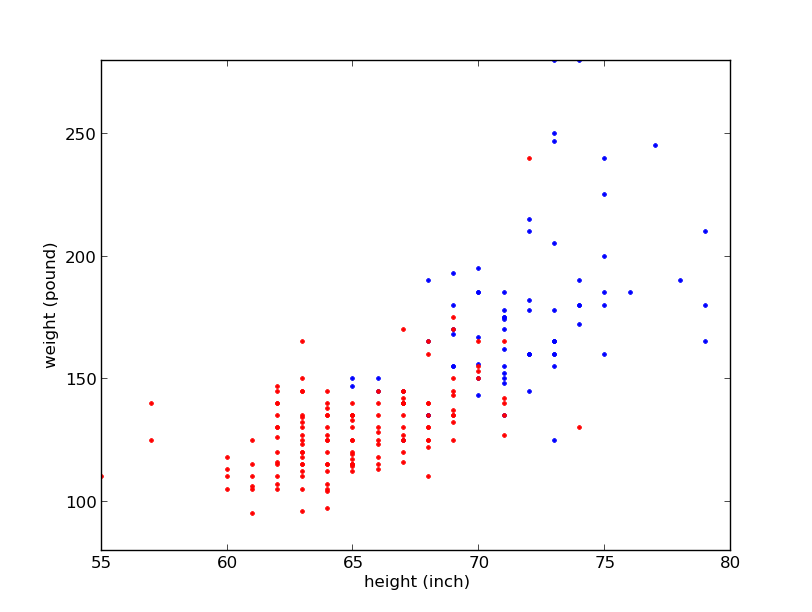
\includegraphics[height=6cm]{plotbio.png}

Bu grafik kadinlar ve erkeklerin boy (height) ve kilolarini (weight) iceren
bir veri setinden geliyor, veri setinde erkekler ve kadinlara ait olan
olcumler onceden isaretlenmis / etiketlenmis (labeled), biz de bu
isaretleri kullanarak kadinlari kirmizi erkekleri mavi ile grafikledik. Ama
bu isaretler / etiketler verilmis olsun ya da olmasin, kavramsal olarak
dusunursek eger bu veriye bir dagilim uydurmak (fit) istersek bir karisim
kullanilmasi gerekli, cunku iki tepe noktasiyle daha rahat temsil
edilecegini dusundugumuz bir durum var ortada.

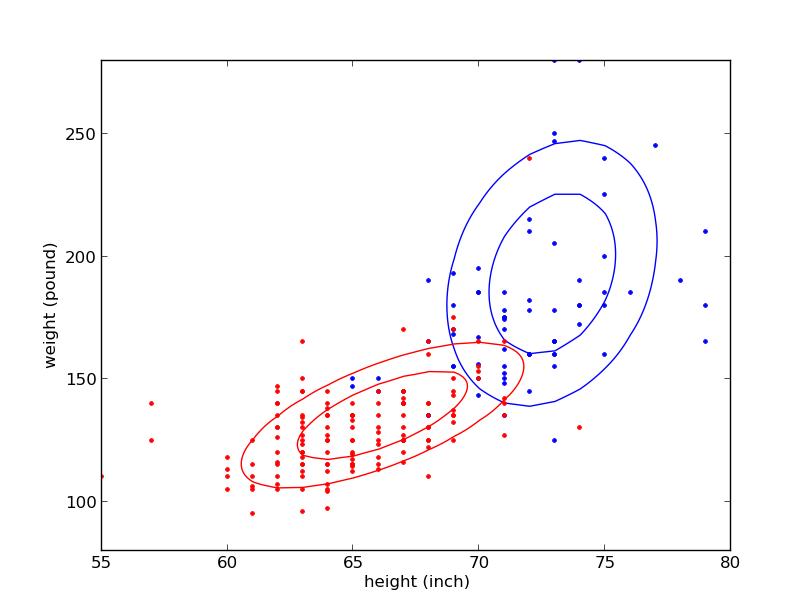
\includegraphics[height=6cm]{plotbio_cluster.png}

Bu karisim icindeki Gaussian'lari ustteki gibi cizebilirdik (gerci ustteki
aslinda ileride yapacagimiz net bir hesaptan bir geliyor, ona birazdan
geliyoruz, ama ciplak gozle de bu sekil uydurulabilirdi). Modeli kontrol
edelim, elimizde bir karisim var, nihai olasilik degeri $p(x)$'i nasil
kullaniriz? Belli bir noktanin olasiligini hesaplamak icin bu noktayi her
iki Gaussian'a teker teker geceriz (ornekte iki tane), ve gelen olasilik
sonuclarini karisim oranlari ile carparak toplariz.

Agirliklar sayesinde iki sey elde ediyoruz 1) karisim entegre edilince hala
1 degeri cikiyor zaten bir dagilimin uymasi gereken sartlardan biri bu 2)
kesisim olan bolgelerde her iki Gaussian buyuk bir deger verebilir, o zaman
agirliklar devreye girer, ve nihai olasilik, agirliklara gore carpilip
toplanan bir sonuc olur. Bu bolgelerde bir Gaussian'in agirliginin
digerinden fazla olmasinin da ozel bir anlami var, demek ki o bolgede
agirligi fazla olan Gaussian daha fazla noktaya sahip (verisel olarak), ki
o zaman o bolgedeki bir noktanin olasiligi sorulunca, agirligi fazla olan
Gaussian daha yuksek bir olasilik degeri geri dondurmeli.

Kesisme olmayan bolgeler zaten pek onemli degil, o noktalarin olasilik
degeri zaten agirlikla tek bir Gaussian'dan geliyor olacak, cunku diger
Gaussian o bolge icin sifira yakin bir deger verir, ve bu sifira yakin
deger toplamda zaten bir fark yaratmayacak.

Etiketler Bilin\textbf{mi}yorsa

Simdi veriyi modellemenin otesinde, biraz daha analitik, daha makine
ogrenimi ile alakali ihtiyaclara gelelim. Eger etiketler bize onceden
verilmemis olsaydi, hangi veri noktalarinin kadinlara, hangilerinin
erkeklere ait oldugunu bilmeseydik o zaman ne yapardik? Bu veriyi
grafiklerken etiketleri renkleyemezdik tabii ki, soyle bir resim
cizebilirdik ancak,

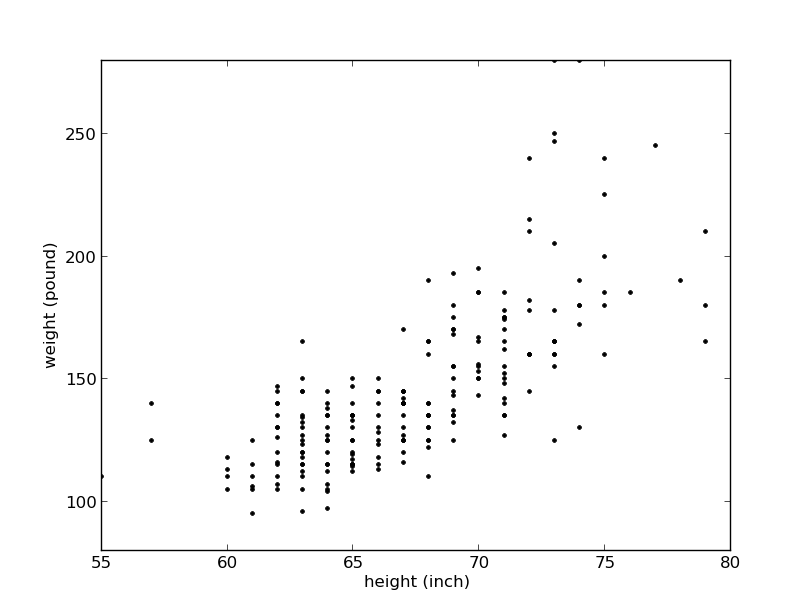
\includegraphics[height=6cm]{plotbio2.png}

Fakat yine de sekil olarak iki kumeyi gorebiliyoruz. 

Acaba oyle bir makine ogrenimi algoritmasi olsa da, biz bir karisim
oldugunu tahmin edip, sonra o karisimi veriye uydururken, etiket
degerlerini de kendiliginden tahmin etse? Bu tam bir veri madenciligi
denemesi olurdu.

Bu ise baslamadan once etiketler ile karisimlarin arasindaki baglantiyi
gorelim. Her nokta icin bilinen / bilinmeyen etiket kavramindan,
matematiksel olarak direk karisimlara gecis yapabilmemiz lazim.

Diyelim ki her nokta icin $0/1$ degerini tasiyabilecek ``gizli'' bir $z$
rasgele degiskeni var, o zaman $p(x)$'i su sekilde acabiliriz

\[ p(x) = \sum_z p(x,z) \]

Bu mantikli degil mi? Ortak dagilim $p(x,z)$ icinden $p(x)$'i cekip
cikarmak, $p(x,z)$ icin bir bilesen (marginal) hesabi yapmak demektir, o
zaman ortak dagilimin icindeki tum $z$ degerlerini toplamak gerekir. Devam
edelim, Bayes Teorisi'ni kullanarak

\[ = \sum_z p(x,z) = \sum_z  p(z)p(x|z) \]

elde ederiz. Burada $p(z)$, yani $z$'nin 0/1 degerine ``sahip olup
olmadiginin olasiligi'' bizi $\pi_z$'ye goturur, yani

\[ \sum_z  p(z)p(x|z) = \sum_z  \pi_zN_z(x | \mu_z,\sigma_z) \]

Unutmayalim, $z$ bir rasgele degisken, ve sahip oldugu olasiliga gore, her
veri noktasi icin, 0 ya da 1 uretiyor. $p(z)$ dedigimiz zaman $z$ tek
basina, baska hicbir parametre ona gecilmiyor, o zaman zaten tanim
itibariyle ``ta en bastan belirli'' bir olasiliktan baska bir seye sahip
olamaz, bu da karisim orani $\pi_z$'den baskasi degildir. 

Simdi notasyonu biraz daha berraklastiralim. Oncelikle, ozellikle Bayes
modelleri iceren formulasyonlarda, $p(x)$, $p(z)$ gibi kullanimlar gorulur,
fakat aslinda orada iki tane farkli yogunluk fonksiyonu (density function)
kastedilir, $p_x(x)$ ve $p_z(z)$. Surekli $p$ kullanilan turden kullanimin
biraz ustunkoru (sloppy) oldugu dogrudur, ama literaturu takip eden herkes
bunun nereden geldigini bilir, sadece konuya ilk baslayanlar icin biraz kafa
karistirici olabiliyor.













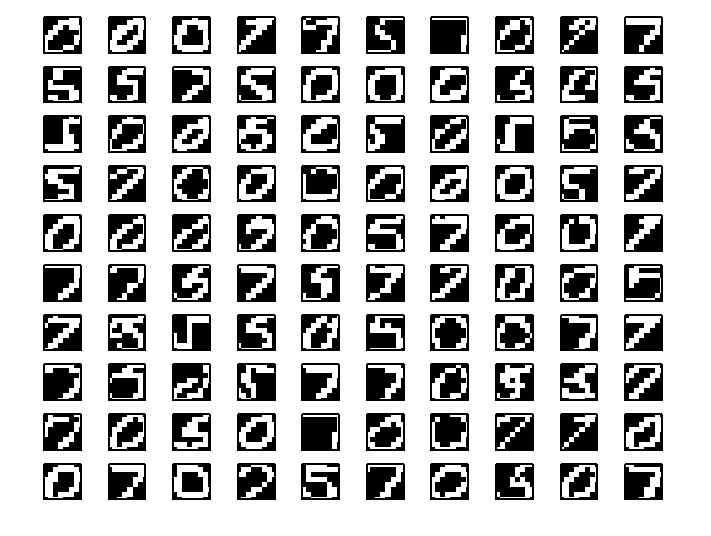
\includegraphics[height=6cm]{digits.png}




\end{document}
